\chapter{流体中的声波}\label{ch:b2:sound-waves}

数一数闪电与雷声之间的秒数，再除以三，
所得即为距离，单位为千米。声音在空气中
每秒传播约三分之一千米，在水中约每秒一千五百米，
超声扫描仪测量人体内部回波的时间，精确到百万分之一秒，
由此绘出图像。本章把
\cref{ch:b2:euler-bernoulli,ch:b2:fluid-kinematics}中的流体力学方法
应用于一团受微小压强扰动的静止流体，
并再次得到达朗贝尔方程：声速、携带能量的是什么、
声音有多响、声音如何在空间中传播，
以及警笛经过时音调为何变化。

\section{声学近似}

\begin{definition}[声学扰动]\label{def:b2:sound-waves:approximation}
\index{声学近似}\index{声压}
一团静止流体，压强均匀为 $P_0$，密度为 $\rho_0$，
受到扰动：$P = P_0 + p(M, t)$，$\rho = \rho_0 + \rho_1(M, t)$，速度
为 $\vect v(M, t)$。\emph{声学近似}只保留
微小量 $p$（\emph{声压}）、$\rho_1$ 与 $\vect v$ 的一阶项，
并要求 $|p| \ll P_0$，$|\rho_1| \ll \rho_0$，$v \ll c$，
且每个流体微团所经历的过程进行得极快，
以至于不与外界交换热量：该过程为\emph{等熵的}，
压缩系数为 $\chi_S = \frac1\rho\bigl(\frac{\partial\rho}{\partial P}\bigr)_S$。
忽略重力。
\end{definition}

\begin{theorem}[声波]\label{thm:b2:sound-waves:equation}
\index{声速}\index{波动方程（声学）}
一阶近似下，欧拉方程、质量守恒与等熵律
分别写为
\[
\rho_0\frac{\partial\vect v}{\partial t} = -\operatorname{\vect{grad}}p , \qquad
\frac{\partial\rho_1}{\partial t} + \rho_0\operatorname{div}\vect v = 0 , \qquad
\rho_1 = \rho_0\chi_Sp ,
\]
二者联立即得声压满足的波动方程，
\[
\Delta p = \frac1{c^2}\frac{\partial^2p}{\partial t^2} , \qquad
c = \frac1{\sqrt{\rho_0\chi_S}} ,
\]
（$\rho_1$ 与 $\vect v$ 满足同样的方程）。对于理想气体，$\chi_S =
1/\gamma P_0$，且
\[
c = \sqrt{\frac{\gamma P_0}{\rho_0}} = \sqrt{\frac{\gamma RT}{M}} :
\]
在 \qty{20}{\degreeCelsius} 的空气中为 \qty{343}{m/s}，温度每升高一开尔文
增加 \qty{0.6}{m/s}；氦气中为 \qty{1000}{m/s}，水中为 \qty{1480}{m/s}（$\chi_S =
\qty{4.5e-10}{Pa^{-1}}$）。
\end{theorem}

\begin{proof}
欧拉方程：对流项 $\rho(\vect v\cdot\operatorname{\vect{grad}})\vect v$
是二阶小量，$\rho\,\partial_t\vect v \approx \rho_0\,\partial_t\vect v$，且
$\operatorname{\vect{grad}}P = \operatorname{\vect{grad}}p$。质量守恒：$\partial_t\rho +
\operatorname{div}(\rho\vect v) \approx \partial_t\rho_1 + \rho_0\operatorname{div}\vect v$。
等熵关系：$\dd\rho = \rho\chi_S\,\dd P$，取一阶近似。对第一式取
散度，对第二式取时间导数：
$\rho_0\partial_t\operatorname{div}\vect v = -\Delta p = -\partial_t^2\rho_1 = -\rho_0\chi_S
\partial_t^2p$。对理想气体，$PV^\gamma$ 沿等熵过程为常数，
由此得 $\dd\rho/\rho = \dd P/\gamma P$，于是 $\chi_S = 1/\gamma P$，
且 $P_0/\rho_0 = RT/M$。
\end{proof}

\begin{remark}[为何是等熵的]\label{rem:b2:sound-waves:laplace}
牛顿用等温压缩系数计算声速，
得 $\sqrt{P_0/\rho_0} = \qty{290}{m/s}$，偏低 $15\%$；拉普拉斯发现
压缩过程太快，热量来不及在较热的波峰与较冷的
波谷之间流动——一个周期内，热量只扩散几微米
（见\cref{ch:b2:heat-conduction}），与一个波长相比几乎可以忽略——
因此过程为绝热且可逆的，$\gamma$ 随之出现。
因此声速可直接用于测定 $\gamma$：空气为 $1.40$，
氩为 $1.67$。
\end{remark}

\begin{omfigure}
\begin{tikzpicture}[font=\small, x=1cm, y=1cm, >=Stealth]
  \begin{scope}
    \draw[thick] (-3.2,-0.8) rectangle (3.2,0.8);
    \fill[omDef!25] (-0.6,-0.8) rectangle (0.6,0.8);
    \fill[omDef!8] (-0.35,-0.8) rectangle (0.95,0.8);
    \draw[omDef, dashed] (-0.35,-0.8) -- (-0.35,0.8) (0.95,-0.8) -- (0.95,0.8);
    \draw[omThm, very thick, ->] (-1.6,0) -- (-0.65,0) node[above, font=\footnotesize, pos=0.3] {$P(x)S$};
    \draw[omThm, very thick, ->] (1.6,0) -- (0.65,0) node[above, font=\footnotesize, pos=0.3] {$P(x+\dd x)S$};
    \node[font=\footnotesize] at (-0.6,-1.1) {$x$}; \node[font=\footnotesize] at (0.65,-1.1) {$x + \dd x$};
    \draw[omDef, ->] (-0.6,1.05) -- (-0.35,1.05) node[above, font=\footnotesize, pos=1.4] {$\xi(x)$};
    \node[font=\footnotesize] at (0,-1.7) {$\rho_0\,\partial_t v = -\partial_x p$, \quad $\rho_1 = -\rho_0\,\partial_x\xi = \rho_0\chi_S\,p$};
  \end{scope}
  \begin{scope}[xshift=8.2cm]
    \foreach \x in {-2.6,-2.45,...,2.6} {
      \pgfmathsetmacro{\d}{0.18*sin(deg(2.4*\x))}
      \draw[omDef, thick] ({\x+\d},-0.8) -- ({\x+\d},0.8);
    }
    \node[font=\scriptsize] at (-1.6,-1.1) {密部}; \node[font=\scriptsize] at (0,-1.1) {疏部}; \node[font=\scriptsize] at (1.6,-1.1) {密部};
    \draw[omThm, thick, ->] (-0.4,1.1) -- (0.8,1.1) node[right, font=\footnotesize] {$c$};
    \node[font=\footnotesize] at (0,-1.7) {平面声波：流体层时而挤聚，时而散开};
  \end{scope}
\end{tikzpicture}

{\small 左图：一层流体发生位移 $\xi(x, t)$，
受其两面的压强作用；其压缩决定了声压。
右图：平面声波——密部与疏部交替分布，
以 $c$ 传播，流体本身沿传播方向来回振动
（纵波）。}
\end{omfigure}

\section{平面波、阻抗、强度}

\begin{proposition}[平面声行波]\label{prop:b2:sound-waves:plane}
\index{声阻抗}\index{声强}\index{能量密度（声学）}
对于平面波 $p = f(x - ct)$，沿 $+x$ 方向传播，流体
速度沿 $x$ 方向，与声压同相，且
\[
p = Z\,v , \qquad Z = \rho_0c = \sqrt{\rho_0/\chi_S} ,
\]
其中 $Z$ 为介质的\emph{声阻抗}
（\unit{kg.m^{-2}.s^{-1}}）：空气为 \qty{410}{kg.m^{-2}.s^{-1}}，
水为 \qty{1.5e6}{kg.m^{-2}.s^{-1}}，软组织为 $\sim\qty{1.6e6}{kg.m^{-2}.s^{-1}}$，
钢为 \qty{4e7}{kg.m^{-2}.s^{-1}}。声波携带能量密度和
声强（沿 $+x$ 方向，单位面积上的功率）
\[
e = \tfrac12\rho_0v^2 + \tfrac12\chi_Sp^2 , \qquad I = p\,v ,
\]
它们满足 $\partial_te + \partial_xI = 0$；对于行波，
$e$ 的两半相等，且 $I = p^2/Z = Zv^2$。正弦波的
压强振幅为 $p_m$，其平均声强为 $\langle I\rangle = p_m^2/2Z$。
\end{proposition}

\begin{proof}
对于 $p = f(x - ct)$，$\rho_0\partial_tv = -\partial_xp = f'/c\cdot c\dots$：精确地说，
$\rho_0\partial_tv = -f'(x - ct)$，且 $v = f(x - ct)/\rho_0c$ 满足该式。$e$ 的势能项是压缩流体所储存的功
（单位体积的等熵压缩，压缩量 $\dd V/V = -\chi_S\,\dd p$
所储存的能量为 $\int p\,\chi_S\dd p = \tfrac12\chi_Sp^2$）；$I$ 为
压力 $pS$ 对前方以速度 $v$ 运动的流体所做功的功率，按单位面积计。
平衡关系：$\partial_te = \rho_0v\partial_tv + \chi_Sp\partial_tp = -v\partial_xp - p\partial_xv =
-\partial_x(pv)$，
由两个线性化方程得出。
\end{proof}

\begin{definition}[声级]\label{def:b2:sound-waves:decibel}
\index{分贝}\index{声级}\index{听阈}
平均强度为 $I$ 的波的\emph{声级}定义为
\[
L = 10\log_{10}\frac I{I_0} \ \text{dB} , \qquad I_0 = \qty{1e-12}{W/m^2}
\]
——\qty{1}{kHz} 处的听阈，在空气中对应于
压强振幅 $p_0 \approx \qty{2e-5}{Pa}$（均方根值）$= 2 \times 10^{-10}$
个大气压。强度加倍则增加 \qty{3}{dB}；强度增至十倍，增加 \qty{10}{dB}；
压强振幅增至百倍，增加 \qty{40}{dB}。安静的房间
\qty{30}{dB}，交谈 \qty{60}{dB}，繁忙的街道 \qty{80}{dB}，摇滚音乐会
\qty{110}{dB}，疼痛 \qty{120}{dB}（$I = \qty{1}{W/m^2}$，$p_m = \qty{29}{Pa}$）。
\end{definition}

\begin{example}[声音有多微弱]\label{ex:b2:sound-waves:small}
在听阈处，\qty{1}{kHz}：$p_m = \qty{2.8e-5}{Pa}$，$v_m = p_m/Z =
\qty{7e-8}{m/s}$，位移振幅 $\xi_m = v_m/\omega =
\qty{1e-11}{m}$——约为原子直径的十分之一：鼓膜能够探测到
比原子还小的运动。在 \qty{120}{dB} 时，$\xi_m = \qty{11}{\micro m}$，
仍然不可见，且 $p_m/P_0 = 3 \times 10^{-4}$：即使是最响的声音
也只是微小的扰动，这正是线性理论如此有效的原因。
\end{example}

\begin{omfigure}
\begin{tikzpicture}
\begin{axis}[omaxis, axis x line=middle, axis y line=left, width=7.4cm, height=4.2cm,
    xlabel={$x$}, ylabel={}, xmin=0, xmax=6.6, ymin=-1.3, ymax=1.4, xtick=\empty, ytick=\empty, samples=100,
    xlabel style={at={(axis description cs:1.0,0.5)}, anchor=west},
    legend style={font=\scriptsize, at={(0.5,1.02)}, anchor=south, legend columns=3, draw=none, fill=none}]
  \addplot[omThm, thick, domain=0:6.28] {sin(deg(x))};
  \addplot[omDef, thick, dashed, domain=0:6.28] {sin(deg(x))};
  \addplot[omProp, thick, domain=0:6.28] {cos(deg(x))};
  \legend{$p$, $v = p/Z$, $\xi$}
\end{axis}
\end{tikzpicture}
\hfill
\begin{tikzpicture}[font=\small, x=1cm, y=1cm, >=Stealth]
  \draw[thick, ->] (0,0) -- (0,4.4);
  \foreach \l/\t in {0/听阈, 1/树叶沙沙声, 2/安静的房间, 3/交谈, 4/繁忙的街道, 5/\qty{10}{m} 外的卡车, 6/摇滚音乐会, 7/痛阈} {
    \pgfmathsetmacro{\y}{0.6*\l}
    \draw (-0.1,\y) -- (0.1,\y);
    \node[anchor=east, font=\scriptsize] at (-0.15,\y) {\pgfmathparse{int(20*\l)}\pgfmathresult~dB};
    \node[anchor=west, font=\scriptsize] at (0.15,\y) {\t};
  }
  \node[font=\scriptsize, anchor=south] at (0,4.45) {$I$（每档 $\times 100$）};
\end{tikzpicture}

{\small 左：平面行进声波中，超压与流体速度同相，
位移滞后四分之一周期。右：分贝刻度——每 \qty{20}{dB} 一档，
强度乘以一百，
压强振幅乘以十。}
\end{omfigure}

\section{球面波}

\begin{proposition}[球面波与平方反比律]\label{prop:b2:sound-waves:spherical}
\index{球面波}\index{平方反比律（声）}
一个向各个方向均匀辐射的小声源，
产生如下球面波
\[
p(r, t) = \frac{A}{r}\,f\Bigl(t - \frac rc\Bigr) ,
\]
其振幅按 $1/r$ 衰减，强度按 $1/r^2$ 衰减：
对于声功率为 $\mathcal P$ 的声源，$I = \mathcal P/4\pi r^2$，即\
距离每增大一倍，强度变化 $-\qty{6}{dB}$。远离声源处，
波局部为平面波，且 $v = p/Z$ 沿径向。
\end{proposition}

\begin{proof}
在球坐标中，对仅依赖于 $r$ 的函数，$\Delta p =
\frac1r\frac{\partial^2(rp)}{\partial r^2}$（在本阶段不加证明地承认；见\cref{ch:b2:maxwell-equations}），
故 $u = rp$ 满足一维波动方程 $\partial_r^2u = \partial_t^2u/c^2$，
由此得出向外传播的波 $u = Af(t - r/c)$。穿过
半径为 $r$ 的球面的功率为 $4\pi r^2I$，若无吸收则为常量。
\end{proof}

\begin{example}[警笛与交谈]\label{ex:b2:sound-waves:siren}
一个功率为 \qty{10}{W} 的警笛：$I = 10/4\pi r^2$，在 \qty{1}{m} 处为 \qty{0.8}{W/m^2}（\qty{119}{dB}，
疼痛），在 \qty{100}{m} 处为 \qty{79}{dB}，在 \qty{1}{km} 处为 \qty{59}{dB}——在城市上空仍可听见。
人声的辐射功率约为 \qty{10}{\micro W}：在 \qty{1}{m} 处为 \qty{60}{dB}，
在 \qty{10}{m} 处为 \qty{40}{dB}。空气也会吸收声音（高频声吸收更多，
在 \qty{10}{kHz} 时每百米衰减数分贝），这正是
远处雷声听起来低沉的原因。
\end{example}

\section{多普勒效应}

\begin{theorem}[多普勒效应]\label{thm:b2:sound-waves:doppler}
\index{多普勒效应}
声源以频率 $f$ 发声，并沿其与观察者的连线以速率 $v_s$ 运动，
观察者以速率 $v_o$ 运动，两速率在相互靠近时取正值；
声音在静止空气中的速率为 $c$。
观察者接收到的频率为
\[
f' = f\,\frac{c + v_o}{c - v_s} .
\]
运动的声源使其前方波前变密（$\lambda' = (c - v_s)/f$），
后方波前变疏；运动的观察者遇到波前的
速率为 $(c + v_o)/\lambda$。当 $v_s, v_o \ll c$ 时，二者均给出 $\Delta f/f \approx
(v_s + v_o)/c$。
\end{theorem}

\begin{proof}
运动源：在 $t$ 与 $t + 1/f$ 时刻发出的波前，沿运动方向
相隔 $c/f - v_s/f$，故前方波长为
$\lambda' = (c - v_s)/f$，固定观察者接收到的频率为
$c/\lambda'$。运动观察者：波长为 $\lambda = c/f$，波前以
相对速率 $c + v_o$ 经过。综合即得。
\end{proof}

\begin{omfigure}
\begin{tikzpicture}[font=\small, x=1cm, y=1cm, >=Stealth]
  \begin{scope}
    \foreach \i in {0,1,2,3,4} {
      \pgfmathsetmacro{\r}{0.45*(5-\i)}
      \pgfmathsetmacro{\cx}{0.27*\i-0.23}
      \draw[omDef, thick] (\cx,0) circle (\r);
    }
    \fill[omThm] (1.12,0) circle (2pt);
    \draw[omThm, thick, ->] (1.12,0.15) -- (1.9,0.15) node[above, font=\footnotesize] {$v_s$};
    \node[font=\footnotesize] at (2.0,-2.45) {前方：$\lambda' < \lambda$};
    \node[font=\footnotesize] at (-1.5,-2.45) {后方：$\lambda' > \lambda$};
    \node[font=\footnotesize] at (0.4,-3.2) {$f' = f\,\dfrac{c + v_o}{c - v_s}$};
  \end{scope}
  \begin{scope}[xshift=8.2cm]
    \foreach \i in {0,1,2,3,4} {
      \pgfmathsetmacro{\r}{0.4*(5-\i)}
      \pgfmathsetmacro{\cx}{0.6*\i-1.12}
      \draw[omDef, thick] (\cx,0) circle (\r);
    }
    \fill[omThm] (1.88,0) circle (2pt);
    \draw[omThm, thick, ->] (1.88,0.15) -- (2.7,0.15) node[above, font=\footnotesize] {$v > c$};
    \draw[omProp, thick] (1.88,0) -- (-0.36,2.0); \draw[omProp, thick] (1.88,0) -- (-0.36,-2.0);
    \draw (0.9,0) arc[start angle=180, end angle=138, radius=0.98] node[left, font=\footnotesize, xshift=-1pt] {$\theta$};
    \node[font=\footnotesize] at (0.3,-3.2) {马赫锥：$\sin\theta = c/v$};
  \end{scope}
\end{tikzpicture}

{\small 左：运动源的波前在前方挤压、后方稀疏，
接近时音调升高，远离时音调降低。右：速度大于声速的源
把波前抛在身后，这些波前的包络即马赫锥，
在地面上听到的是爆鸣声。}
\end{omfigure}

\begin{example}[警笛、测速雷达、红细胞]\label{ex:b2:sound-waves:dopplerex}
救护车警笛频率为 \qty{700}{Hz}，以 \qty{25}{m/s} 的速率驶过时：接近时为 \qty{755}{Hz}，
远离时为 \qty{651}{Hz}——音高下降了六分之一个八度，
即人们熟悉的“呜哇”声中那一段下降。警用测速雷达测量的是同一效应，
所用的是被汽车反射的 \qty{24}{GHz} 无线电波（
汽车接收并再发射，频移两次）：$\Delta f = 2fv/c =
\qty{4.8}{kHz}$，速率为 \qty{30}{m/s}。以 \qty{5}{MHz} 的超声探头对准
一条动脉时，接收到的血细胞回波频移为 $\Delta f = 2fv\cos\theta/c \approx \qty{1.6}{kHz}$
（取血流速率 \qty{0.5}{m/s}，角度 \qty{60}{\degree}）：可听见的哨声，其音调即为
血流速率。远离我们的星系的谱线则向
红端移动，$\Delta\lambda/\lambda = v/c$——该式适用于低速的光，
速度较高时需加相对论修正。
\end{example}

\begin{remark}[超音速]\label{rem:b2:sound-waves:mach}
\index{马赫锥}\index{音爆}
当 $v_s > c$ 时公式失效（前方 $f' < 0$）：没有声音先于
声源到达。沿路径发出的波前具有锥形包络，
其半顶角 $\theta$ 满足 $\sin\theta = c/v_s$（\emph{马赫锥}）；
锥面所携带的压强跃变即音爆，它
只有在飞机飞过之后才会到达地面上的听者——
在马赫数为 $2$、高度为 \qty{10}{km} 时，$\theta = \qty{30}{\degree}$，音爆
在飞机正上方经过后约 $10\,\text{千米}/\tan\theta/v_s \approx \qty{25}{s}$ 才抵达。
子弹的破空声与鞭梢的爆鸣，都来自同一个锥面。
\end{remark}

\begin{method}[声学中的数量级]\label{met:b2:sound-waves:method}
已知声强级 $L$：$I = I_0\,10^{L/10}$；再由 $p_m = \sqrt{2ZI}$，
$v_m = p_m/Z$，$\xi_m = v_m/\omega$；若声源向各个方向辐射，其功率为 $4\pi r^2I$，
在坚硬地面上则减半（地面将其反射入半空间）。
由 $r_1$ 变到 $r_2$ 时，$L$ 改变
$20\log_{10}(r_1/r_2)$。叠加 $n$ 个相同的不相干声源，将增加
$10\log_{10}n$；两个在某点同相的相干声源则增加 \qty{6}{dB}。
\end{method}

\section{练习}

\begin{exercise}[$\star$]\label{exo:b2:sound-waves:1}
求空气（$\gamma = 1.40$，$M = \qty{29}{g/mol}$）在
\qty{0}{\degreeCelsius}、\qty{20}{\degreeCelsius} 及 \qty{-50}{\degreeCelsius} 时的声速，
（\qty{10}{km} 高度）；氦气（$\gamma = 1.67$，$M = \qty{4}{g/mol}$）和
二氧化碳（$\gamma = 1.30$，$M = \qty{44}{g/mol}$）在 \qty{20}{\degreeCelsius} 时的声速。
为什么吸入氦气后，说话声音会变尖？
\end{exercise}

\begin{exercise}[$\star$]\label{exo:b2:sound-waves:2}
求 \qty{60}{dB}、\qty{500}{Hz} 的谈话声在空气中的强度、压强
振幅、速度振幅及位移振幅（空气的声阻抗
为 $Z = \qty{410}{kg.m^{-2}.s^{-1}}$）。同样求 \qty{120}{dB} 时的结果。
求两人同时说话与一百人同时说话时的声强级。
\end{exercise}

\begin{exercise}[$\star$]\label{exo:b2:sound-waves:3}
一个扬声器向各方向等量辐射功率为 \qty{1.0}{W} 的声波。
求在 \qty{1}{m}、\qty{10}{m}、\qty{100}{m} 处的声强与声强级；求声强级
降至 \qty{60}{dB} 的距离；求在 \qty{30}{m} 处达到 \qty{100}{dB} 所需的功率
（露天音乐会）。
\end{exercise}

\begin{exercise}[$\star$]\label{exo:b2:sound-waves:4}
闪电后 \qty{4.5}{s} 听到雷声：求距离。一艘船的汽笛声
经悬崖反射，\qty{3.0}{s} 后听到回声：求距离。声呐：来自
海底的回波在 \qty{2.4}{s} 后返回（$c = \qty{1500}{m/s}$）：求水深。一个
\qty{5}{MHz} 的超声回波在组织中经 \qty{130}{\micro s} 后返回
（\qty{1540}{m/s}）：求深度。
\end{exercise}

\begin{exercise}[$\star\star$]\label{exo:b2:sound-waves:5}
一列火车的汽笛频率为 \qty{500}{Hz}，$c = \qty{340}{m/s}$。(a) 站台上的人
在火车以 \qty{40}{m/s} 驶近时所听到的频率，
以及火车驶过之后所听到的频率。(b) 人乘坐的火车朝汽笛驶去，
速率为 \qty{40}{m/s}，汽笛静止；随后两者以 \qty{40}{m/s} 的速率相向运动，
与相对速率为 \qty{80}{m/s} 而一方静止的情形作比较。
(c) 汽笛所在火车上的司机，听到的
来自前方墙壁回声的频率。
\end{exercise}

\begin{exercise}[$\star\star$]\label{exo:b2:sound-waves:6}
对于压强振幅为 \qty{1.0}{Pa}、频率为 \qty{1}{kHz} 的声波，计算
空气中的速度振幅与位移振幅、声强及声强级，
水中（$Z = \qty{1.5e6}{kg.m^{-2}.s^{-1}}$）与钢中
（$\qty{4e7}{kg.m^{-2}.s^{-1}}$）的相应量。相同压强下，声强却相差悬殊：
请评论。（水下声级以 \qty{1}{\micro Pa} 为参考给出：在此标度下，
\qty{1}{Pa} 相当于多少？）
\end{exercise}

\begin{exercise}[$\star\star$]\label{exo:b2:sound-waves:7}
(a) 求空气在 \qty{20}{\degreeCelsius} 下的牛顿等温声速 $\sqrt{P_0/\rho_0}$
（$\rho_0 = \qty{1.20}{kg/m^3}$）及拉普拉斯修正。
(b) 实测：空气中为 \qty{343}{m/s}，氩气（$M = \qty{40}{g/mol}$）中为 \qty{323}{m/s}，
温度均为 \qty{20}{\degreeCelsius}。由此求各自的 $\gamma$，并结合自由度数加以解释。
(c) 估计 \qty{1}{kHz} 的一个周期内热量扩散的距离
（空气的热扩散率为
\qty{2e-5}{m^2/s}），并与波长相比较。
\end{exercise}

\begin{exercise}[$\star\star$]\label{exo:b2:sound-waves:8}
\emph{管风琴管。}在管中，开口端的超压为零，
闭口端的速度为零。(a) 求两端开口的管中驻波，证明其模式为 $f_n = nc/2L$；
一端闭合的管中，
$f_n = (2n - 1)c/4L$。(b) 求基频为 \qty{440}{Hz} 时两种情形下的管长；
(c) 每种管含有哪些谐波？(d) 实际的开口端
位于管外约 $0.6$ 倍半径处（端部修正）：
对于 \qty{4}{cm} 的管，求 $L$ 和 $f$ 的修正量。
\end{exercise}

\begin{exercise}[$\star\star$]\label{exo:b2:sound-waves:9}
一台 \qty{2.0}{kW} 的电动警报器，将其功率的 $20\%$ 转化为声能，
辐射进入半空间（它装在屋顶上）。(a) 求 \qty{100}{m} 处的声强、声强级
及压强振幅。(b) 求痛阈的距离
（\qty{120}{dB}），以及 \qty{70}{dB} 等值线（超出该线即不再令人警觉）的距离。
(c) 空气吸收在该频率下每 100 m 附加 \qty{1}{dB} 的损耗：
此时 \qty{70}{dB} 等值线的距离是多少（数值求解）。(d) 需要多少台
此类警报器才能覆盖半径为 \qty{10}{km} 的城市？
\end{exercise}

\begin{exercise}[$\star\star\star$]\label{exo:b2:sound-waves:10}
\emph{驻声波的能量。}在长为 $L$ 的闭管中
超压为 $p = p_m\cos(kx)\cos(\omega t)$，$k = n\pi/L$。(a) 由线性化欧拉方程求 $v(x,
t)$。(b) 求动能密度与势能密度；
证明二者随时间呈正交振荡，
在空间上相差四分之一波长。(c) 求管中的总能量
（截面为 $S$），并验证其为常量。(d) 平均声强处处为零——
然而能量确实在运动，请描述其运动方式。
\end{exercise}

\begin{exercise}[$\star\star\star$]\label{exo:b2:sound-waves:11}
\emph{声爆。}一架飞机以 $v = 1.6\,c$ 的速度水平飞行，
飞行高度 $h = \qty{12}{km}$，该处 $c = \qty{300}{m/s}$。(a) 由球面波前的包络推导马赫
角。(b) 求飞机头顶经过与地面听到爆声
之间的时间（不计
$c$ 随高度的变化）。(c) 求地面上听到爆声
的条带宽度（飞机飞过时），若锥迹在
航迹两侧 $\pm\qty{30}{km}$ 内可被听到，为何陆地上空的超声速飞行
被禁止？(d) 一颗步枪子弹以 \qty{800}{m/s} 飞行：求其马赫角；
离弹道 \qty{10}{m} 处站立的观察者将先后听到什么，次序如何？
\end{exercise}

\begin{exercise}[$\star\star\star$]\label{exo:b2:sound-waves:12}
\emph{多普勒超声。}一探头以 $f = \qty{5.0}{MHz}$ 的频率向组织中发射声波
（$c = \qty{1540}{m/s}$）；红细胞以速度 $v$ 沿
与声束成 $\theta$ 角的血管运动。(a) 求细胞（运动观察者）接收到的频率。
(b) 细胞将该频率作为运动波源再发射（散射），
求回到探头处的频率；证明 $\Delta f = 2fv\cos\theta/c$（设 $v \ll c$）。(c)
求 $\Delta f$ 在 $v = \qty{0.50}{m/s}$、$\theta = \qty{60}{\degree}$ 时的值；$\theta = \qty{90}{\degree}$ 时
——操作者该怎么办？(d) 探头可分辨 \qty{50}{Hz}：求速度分辨率。
为何要将多普勒信号转换为声音输出，
而不只是显示？
\end{exercise}

\begin{omfigure}
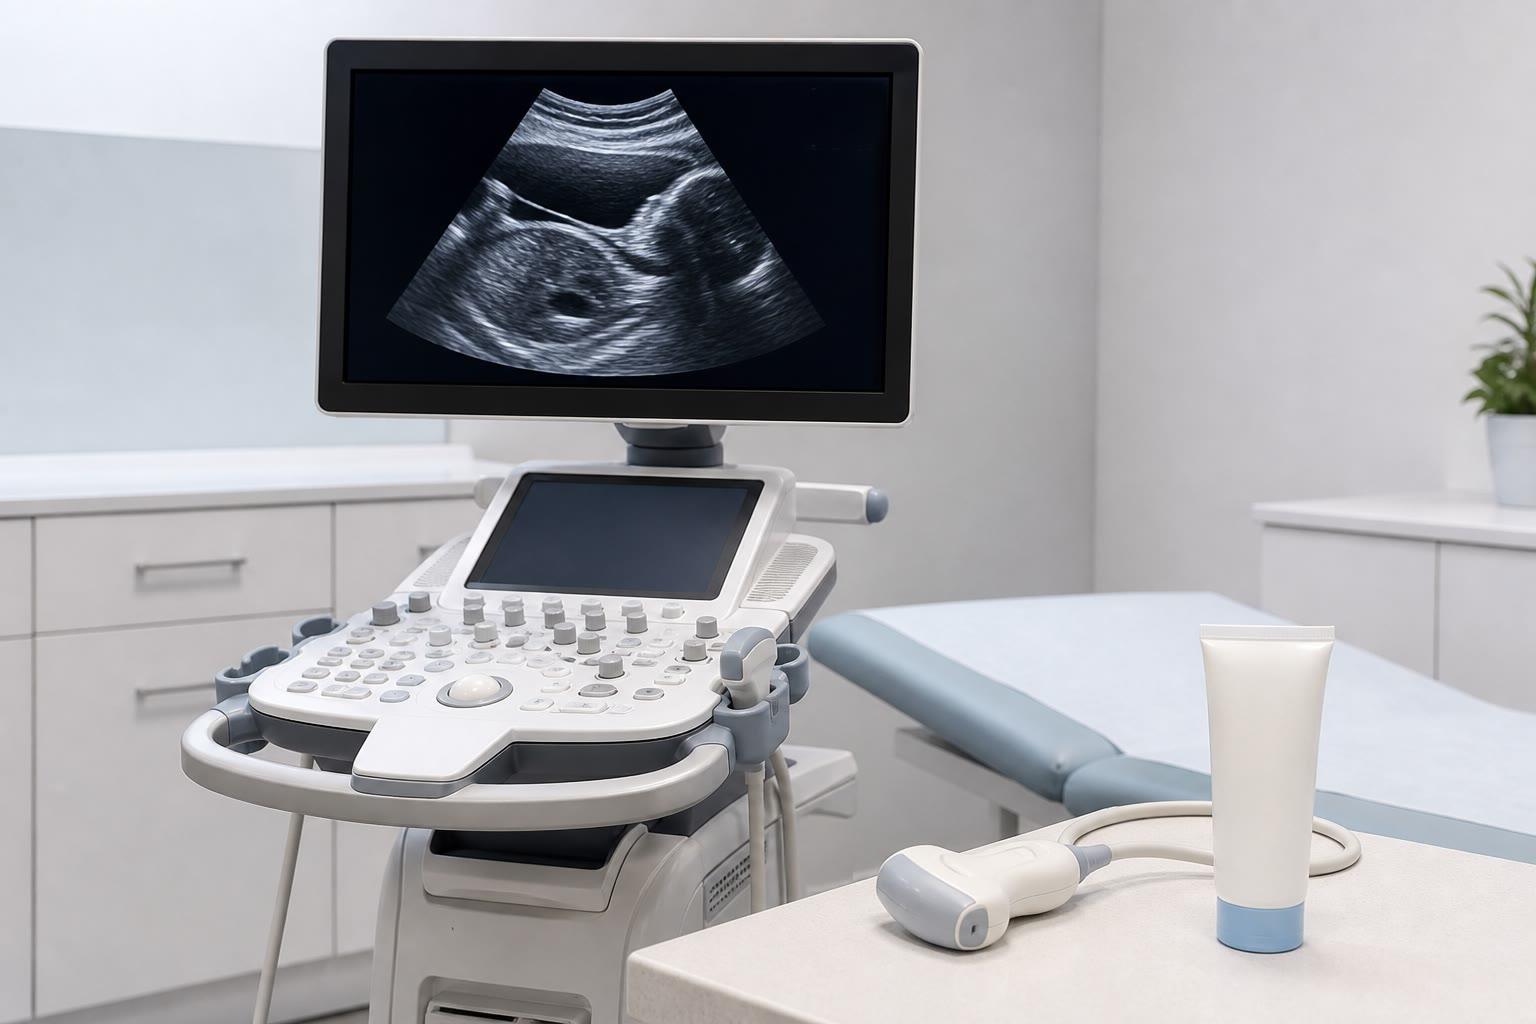
\includegraphics[width=0.58\linewidth]{images/book4/ai/b4-07-ultrasound-probe.jpg}

{\small 超声扫描仪：几兆赫的声波、计时回波以及组织之间的阻抗失配共同绘出图像；耦合凝胶则排除了会把一切都反射回去的空气薄膜。}
\end{omfigure}

\section{问题：从雷声到回波仪}

\begin{problem}[{周末问题——露天中的声音、音乐厅里的声音、
人体内部的声音以及经过的警报器的声音}]
\label{pb:b2:sound-waves:1}

空气：$\gamma = 1.40$，$M = \qty{29}{g/mol}$，$Z = \qty{410}{kg.m^{-2}.s^{-1}}$，
温度为 \qty{15}{\degreeCelsius}；$R = \qty{8.31}{J/(mol.K)}$。

\medskip
\noindent\textbf{第一部分——风暴。}
\begin{enumerate}
  \item 求 \qty{15}{\degreeCelsius} 和 \qty{30}{\degreeCelsius} 时的声速；
        说明“每千米三秒”这一经验规则的依据。
  \item 闪电后 \qty{4.0}{s} 才听到雷声：求雷击点的
        距离。雷声持续数秒，尽管闪电是
        瞬时的：这是为什么？
  \item 在雷击附近，声强级达到 \qty{120}{dB}：求空气的压强振幅
        与速度振幅。
  \item 求一次雷鸣期间墙面每平方米接收的能量，
        该次雷鸣持续 \qty{2}{s}，声强级为 \qty{120}{dB}。
  \item 晴朗的夜晚地面降温，下层空气比上层空气更冷。
        声线在各层之间遵循斯涅耳定律，
        $\sin i/c = $ 常量：向上发出的声线会向下还是向上弯曲？
        为什么夜间及水面上方的远处声音听得特别清楚？
  \item 白天则相反：距离 \qty{3}{km} 处的听者什么也听不到。
        估算水平声线经过
        \qty{3}{km} 后弯曲的角度，设 $c$ 每升高 \qty{500}{m} 下降 \qty{1}{\%}
        （将弯曲视为均匀，即声线为一个圆）。

  \item 空气对高频声的吸收远强于低频声：为何
        远处的雷声呈隆隆低鸣，而近处的雷击则是爆裂声？
\end{enumerate}

\medskip
\noindent\textbf{第二部分——音乐会。}
一台扬声器接收 \qty{100}{W} 的电功率，
其中 $2\%$ 转化为声能，并均匀辐射到其前方的
半空间中。
\begin{enumerate}[resume]
  \item 声功率；\qty{10}{m} 处的声强与声级。
  \item 该处的压强振幅；速度振幅与位移振幅，
        取 \qty{100}{Hz} 时的值。
  \item \qty{1}{m} 处的声级（是否安全？）以及音乐降至
        \qty{60}{dB} 时的距离。
  \item 十台相同的扬声器散布在舞台周围，彼此不同相：
        \qty{10}{m} 处的声级。两台同相馈电的扬声器，
        与听者位于其轴线上且距离相同：该处的声级。
  \item 大厅（体积 \qty{10000}{m^3}）的墙壁与听众共有 \qty{2000}{m^2} 的吸声面，吸收落在其上声音的 $30\%$。
        利用发射功率与吸收功率相等的关系，估算平衡时大厅内储存的声能，
        以及混响时间（音乐停止后声级下降 \qty{60}{dB} 所需的时间），
        其中所用的
        扩散场关系式，
        $I_{\text{壁}} \approx ce/4$ 在本阶段不加证明地承认。
\end{enumerate}

\medskip
\noindent\textbf{第三部分——超声成像仪。}
软组织：$c = \qty{1540}{m/s}$，$Z = \qty{1.6e6}{kg.m^{-2}.s^{-1}}$；骨骼
$Z = \qty{7e6}{kg.m^{-2}.s^{-1}}$；空气 $\qty{400}{kg.m^{-2}.s^{-1}}$。垂直入射时，
界面处反射的压强振幅为入射压强振幅的 $r = (Z_2 -
Z_1)/(Z_2 + Z_1)$ 倍（推导见
\cref{ch:b2:wave-interfaces}）；组织对声的衰减约为
每厘米每兆赫 \qty{0.5}{dB}。
\begin{enumerate}[resume]
  \item 组织中 \qty{3}{MHz}、\qty{5}{MHz}、\qty{10}{MHz} 时的波长；
        每种频率能分辨的最小细节约为一个波长。
  \item 来自深 \qty{12}{cm} 处器官的回波延迟；脉冲可发出的最大速率，
        以使回波不致混淆；形成
        $200$ 条扫描线图像所需的时间。
  \item 压强与能量各自被反射的比例；
        在组织–空气与组织–骨骼界面处，以及在脂肪与肌肉之间界面处的比例（脂肪
        $Z = \qty{1.38e6}{kg.m^{-2}.s^{-1}}$，肌肉
        $\qty{1.70e6}{kg.m^{-2}.s^{-1}}$）。为何要涂耦合剂，为何骨骼
        会形成声影？
  \item 在 \qty{5}{MHz} 时，声束穿过 \qty{2}{cm} 脂肪后到达肌肉：
        从该界面返回探头的能量占发射能量的比例
        （计入反射与往返衰减），以
        分贝表示。
  \item 对第 12 题中的器官，分别计算三种频率下的往返衰减（以分贝计），
        若扫描仪可承受 \qty{80}{dB} 的损耗，
        哪些频率可用？
        并说明分辨率与深度之间的权衡。
  \item 探头以 \qty{5}{MHz} 发射 \qty{1}{\micro s} 的脉冲：
        一个脉冲有多少个波长？
        这如何限制深度方向的分辨率？
  \item 在 \qty{5}{MHz} 下对动脉进行多普勒成像，血流速度为 \qty{0.40}{m/s}，声束与血流方向成
        \qty{60}{\degree}：频移；操作者听到的是什么。
\end{enumerate}

\medskip
\noindent\textbf{第四部分——警笛。}
\begin{enumerate}[resume]
  \item 一辆救护车以 \qty{90}{km/h} 的速度驶过，警笛频率为 \qty{700}{Hz}：
        听到的接近与远离时的频率，
        以及两者之间相差的半音数（半音的比值为 $2^{1/12}$）。
  \item 听者坐在以 \qty{15}{m/s} 的速度驶向迎面而来救护车的汽车中：
        听到的频率。
  \item 在人行道上的听者何时恰好听到
        \qty{700}{Hz}？
  \item 救护车前方的波前：波长；声音相对于救护车
        在前方与后方的速率。
  \item 一支工作在 \qty{24}{GHz} 的雷达测速枪读得来自一辆汽车的 \qty{3.2}{kHz} 频移：
        该汽车的速度（波被移动了两次）。
  \item 总结本题中的六个速率：
        空气中的声速、组织中的声速、救护车的速度、汽车的速度、
        红细胞的速度与光速，以及能统一处理它们的那一个公式。
\end{enumerate}
\end{problem}
